\documentclass[11pt,a4paper]{article}
\usepackage[T1]{fontenc}
\usepackage[utf8]{inputenc}
\usepackage{lmodern}
\usepackage[margin=2.4cm]{geometry}
\usepackage{amsmath,amssymb}
\usepackage{booktabs}
\usepackage{tabularx}
\usepackage{graphicx}
\usepackage{xcolor}
\usepackage{listings}
\usepackage{enumitem}
\usepackage[colorlinks=true,linkcolor=blue!50!black,urlcolor=blue!50!black]{hyperref}

\definecolor{shellbg}{gray}{0.95}
\lstset{
  basicstyle=\ttfamily\small,
  backgroundcolor=\color{shellbg},
  frame=single, rulecolor=\color{gray!60},
  breaklines=true, breakatwhitespace=false,
  columns=fullflexible, keepspaces=true,
  showstringspaces=false,
  xleftmargin=2pt, xrightmargin=2pt,
  aboveskip=6pt, belowskip=6pt,
  literate={~}{{\textasciitilde}}1
}
\newcommand{\f}[1]{\texttt{#1}}          % file / command
\setlist{itemsep=2pt,topsep=4pt}
\setlength{\parindent}{0pt}
\setlength{\parskip}{5pt}
\sloppy

\title{ALF\_SZ: installing, running and analysing\\the two-band spin models in ALF}
\author{Manual for the \f{Hubbard\_Sz} and \f{TwoBand\_Spin} Hamiltonians}
\date{November 2026}

\begin{document}
\maketitle
\tableofcontents

%=======================================================================================
\section{Overview}
%=======================================================================================

This version of ALF (\url{https://github.com/samizwei/ALF}) is the standard ALF code with
two additional Hamiltonians for the two-band model of Christensen \emph{et al.},
Phys.\ Rev.\ Lett.\ \textbf{125}, 247001 (2020). On an $L_1\times L_2$ square lattice with
periodic boundary conditions,
\begin{equation}
  H = H_0 - U\sum_i\sum_{a\in\mathcal A}\bigl(S^a_i\bigr)^2,\qquad
  S^a_i=\sum_{\alpha\beta}c^\dagger_{i\alpha}\sigma^a_{\alpha\beta}d_{i\beta}+\text{h.c.},
\end{equation}
with $\mathcal A=\{z\}$ (Ising, Eq.~(3) of the paper), $\{x,y\}$ (XY) or $\{x,y,z\}$
(Heisenberg). $H_0$ is Eq.~(1) of the paper in real space, with anisotropic hoppings
$t\pm\delta$ and band offset $\mu$; the paper uses $t=1$, $\delta=0.4$, $\mu=-2$.
All three models are free of the sign problem for $U>0$.

\begin{center}
\begin{tabularx}{\textwidth}{llX}
\toprule
\f{ham\_name} & couplings & remarks \\
\midrule
\f{Hubbard\_Sz}   & Ising only & gauge $d_\downarrow\to-d_\downarrow$, $N_\text{SUN}=2$, 2 orbitals/site; $\sim$4$\times$ faster \\
\f{TwoBand\_Spin} & Ising, XY, Heisenberg & chosen by \f{Ham\_Int}; $N_\text{SUN}=1$, 4 orbitals/site \\
\bottomrule
\end{tabularx}
\end{center}

For the Ising coupling both codes give identical results, and both are validated against
exact diagonalisation on $2\times2$ (Sec.~\ref{sec:validation}). The list of all files that
were added to standard ALF is in \f{Infos\_SZ/README.md}.

\paragraph{How ALF works in practice.}
ALF consists of two programs:
\begin{itemize}
  \item \f{Prog/ALF.out}, the QMC simulation. It takes \emph{no command-line arguments}. It
        reads the files \f{parameters} and \f{seeds} from the directory in which it is started
        and writes the Monte Carlo bins into that same directory.
  \item \f{Analysis/ana.out}, the error analysis. It reads the bins and writes means with
        jackknife error bars.
\end{itemize}
A simulation is therefore always ``one directory = one parameter set''. The script
\f{run.sh} (Sec.~\ref{sec:runsh}) automates this, and \f{analyze.py}
(Sec.~\ref{sec:analysis}) turns the output into tables and plots.

%=======================================================================================
\section{Installation}
%=======================================================================================

\subsection{Prerequisites}
\begin{itemize}
  \item A Fortran compiler (\f{gfortran}), \f{make}, and BLAS/LAPACK.
  \item \f{python3}. The build uses it to generate the parameter-reading code of the
        Hamiltonians, and the analysis script needs \f{numpy} (and \f{matplotlib} for plots).
  \item Optional: an MPI library (OpenMPI) for parallel runs.
\end{itemize}

\textbf{macOS} (Homebrew):
\begin{lstlisting}
brew install gcc                 # provides gfortran
brew install lapack              # optional; macOS also ships BLAS/LAPACK (Accelerate)
brew install open-mpi            # optional, for MPI runs
pip3 install numpy matplotlib
\end{lstlisting}
\textbf{Linux} (Debian/Ubuntu):
\begin{lstlisting}
sudo apt install gfortran make liblapack-dev libblas-dev python3-numpy python3-matplotlib
sudo apt install libopenmpi-dev openmpi-bin   # optional, for MPI runs
\end{lstlisting}
On a cluster, load the corresponding modules (compiler, MPI, MKL) instead.

\subsection{Download and compile}
Choose any location for the code, for example \f{\textasciitilde/Codes}:
\begin{lstlisting}
cd ~/Codes
git clone https://github.com/samizwei/ALF.git ALF_SZ
cd ALF_SZ
source configure.sh GNU noMPI      # set compiler and flags (only valid in this shell)
make                               # builds Prog/ALF.out and Analysis/ana.out
\end{lstlisting}
\f{configure.sh} only sets environment variables, so it has to be \emph{sourced} (not executed),
and again in every new terminal before calling \f{make}. Options:
\begin{itemize}
  \item \f{GNU noMPI}: serial build with gfortran (laptop, tests).
  \item \f{GNU MPI}: MPI build with \f{mpifort}; independent Markov chains on each core are
        averaged automatically.
  \item \f{Intel MPI}, \f{Intel noMPI}: Intel compiler and MKL (clusters).
  \item Add \f{HDF5} to write all output into one HDF5 file \f{data.h5} instead of text files.
        This manual assumes text output (no \f{HDF5}), which is what \f{run.sh} and
        \f{analyze.py} read.
\end{itemize}
A successful build ends with the line \f{Link program} and creates
\begin{lstlisting}
ALF_SZ/Prog/ALF.out
ALF_SZ/Analysis/ana.out
\end{lstlisting}

\paragraph{After changing Fortran code} (e.g.\ a Hamiltonian file), run \f{make} again in the
same way (\f{source configure.sh ...} first in a new shell). After pulling new commits with
\f{git pull}, rebuild as well. If the build behaves strangely, start from scratch with
\f{make clean \&\& make}.

\paragraph{Several ALF installations.}
Each ALF folder has its own \f{ALF.out}. The scripts described below always use the
\f{ALF.out} of the folder they are located in. They ignore a global environment variable
\f{ALF\_DIR}, which may point to a different (e.g.\ standard) ALF installation that does
not contain these Hamiltonians.

\subsection{Check the installation}
\begin{lstlisting}
cd ~/Codes/ALF_SZ/Scripts_and_Parameters_files/Hubbard_Sz
./run.sh ~/QMC_runs/Sz_test_2x2 parameters_test_2x2
\end{lstlisting}
This takes about 5\,s and should end with
\begin{lstlisting}
Observable           mean              error
Ener             -31.80983515       0.00718594
Avg. sign          1.00000000       0.00000000
...
\end{lstlisting}
compared with the exact value $-31.80783$. With the same compiler and seeds you should get
the same numbers to all printed digits; on another machine they may differ within the error
bar.

%=======================================================================================
\section{Where to keep code, parameters and data}
\label{sec:layout}
%=======================================================================================

Keep the \textbf{code} and the \textbf{simulation data} in separate folders. Run
directories inside the ALF folder mix data with source files, end up in \f{git status},
and can be removed by clean-up commands. A layout that works well:
\begin{lstlisting}
~/Codes/ALF_SZ/                         <- code (git repository)
    Scripts_and_Parameters_files/
        Hubbard_Sz/      run.sh, analyze.py, parameters templates, seeds
        TwoBand_Spin/    run.sh, parameters templates, seeds

~/QMC_runs/                             <- data (anywhere, e.g. an external disk)
    params/                             <- your parameter files
        Sz_L6_U1_b5
        Heis_L6_U1_b5_dt0.0125
    Sz_L6_U1_b5/                        <- one run directory per parameter set
        parameters                      <- copy actually used by ALF.out
        seeds, info, *_scal, *_eq, ...
    Heis_L6_U1_b5_dt0.0125/
\end{lstlisting}
\begin{itemize}
  \item \textbf{Templates} stay in the ALF folder and are not edited for individual runs.
  \item \textbf{Your parameter files} live next to the data (\f{\textasciitilde/QMC\_runs/params/}).
        You can also keep them in the ALF folder and version them with git; \f{run.sh}
        accepts a parameter file from any path.
  \item Each \textbf{run directory} contains its own copy \f{parameters}, which is the file
        \f{ALF.out} reads. A run directory therefore documents itself.
  \item A useful naming scheme puts the model and the parameters that change into the
        directory name, e.g.\ \f{Heis\_L8\_U2\_b10\_dt0.0125}.
\end{itemize}
\f{\textasciitilde/QMC\_runs} is only an example; any path works, including a folder on an
external disk (\f{/Volumes/MyDisk/QMC\_runs}) or the scratch file system of a cluster.

%=======================================================================================
\section{The parameter file}
\label{sec:parameters}
%=======================================================================================

The parameter file is a set of Fortran namelists. Everything after \f{!} is a comment.
Start from a template:
\begin{lstlisting}
mkdir -p ~/QMC_runs/params
T=~/Codes/ALF_SZ/Scripts_and_Parameters_files
cp $T/Hubbard_Sz/parameters    ~/QMC_runs/params/Sz_L6_U1_b5        # Ising
cp $T/TwoBand_Spin/parameters  ~/QMC_runs/params/Heis_L6_U1_b5      # Ising / XY / Heisenberg
\end{lstlisting}
and change the lines marked \f{<-- SET}. The namelists are:

\begin{description}
\item[\f{\&VAR\_ham\_name}] \f{ham\_name = "Hubbard\_Sz"} or \f{"TwoBand\_Spin"}: selects the model.
\item[\f{\&VAR\_lattice}] \f{L1}, \f{L2}: lattice size. \f{Lattice\_type = "Square"} (only this one is implemented).
\item[\f{\&VAR\_Hubbard\_Sz} / \f{\&VAR\_TwoBand\_Spin}] model parameters, see the table below.
\item[\f{\&VAR\_QMC}] Monte Carlo settings.
\item[\f{\&VAR\_errors}] settings for the analysis program \f{ana.out}.
\end{description}
The name of the model namelist must match \f{ham\_name}: \f{\&VAR\_Hubbard\_Sz} for
\f{Hubbard\_Sz}, \f{\&VAR\_TwoBand\_Spin} for \f{TwoBand\_Spin}.

\begin{center}
\small
\begin{tabularx}{\textwidth}{llX}
\toprule
parameter & default & meaning \\
\midrule
\f{Ham\_Int}   & \f{"Heisenberg"} & \f{TwoBand\_Spin} only: \f{"Ising"}, \f{"XY"} or \f{"Heisenberg"} \\
\f{Ham\_T}     & 1     & hopping $t$ (energy unit) \\
\f{Ham\_delta} & 0.4   & hopping anisotropy $\delta$ \\
\f{Ham\_mu}    & $-2$  & band offset $\mu$ in $-\mu\sum(n^c-n^d)$ \\
\f{Ham\_chem}  & 0     & additional global chemical potential, adds $-\mu_0 N$ \\
\f{Ham\_U}     & 1     & interaction $U$ (use $U>0$; $U<0$ gives a sign problem) \\
\f{Beta}       & 5     & inverse temperature $\beta$ \\
\f{Dtau}       &       & imaginary-time step $\Delta\tau$; number of slices $L_\text{Trot}=\beta/\Delta\tau$ \\
\f{Projector}  & \f{.F.} & \f{.T.}: projective ($T=0$) algorithm with projection length \f{Theta} \\
\f{Symm}       & \f{.T.} & symmetric Trotter decomposition (keep \f{.T.}) \\
\f{N\_part}    & $-1$  & projector only: particle number of the trial state ($<0$: half filling of the two bands) \\
\midrule
\f{NSweep}     & 200   & sweeps per bin; one bin = one stored measurement block \\
\f{NBin}       & 20    & number of bins in this run \\
\f{Nwrap}      & 10    & numerical stabilisation every \f{Nwrap} slices \\
\f{Ltau}       & 0     & 1: also measure time-displaced correlations (\f{*\_tau}); slower \\
\f{CPU\_MAX}   & 0     & $>0$: stop cleanly after this many hours (cluster time limits) \\
\midrule
\f{n\_skip}    & 2     & bins discarded as thermalisation by \f{ana.out} \\
\f{N\_rebin}   & 1     & bins combined into one before the jackknife (autocorrelations) \\
\bottomrule
\end{tabularx}
\end{center}

\paragraph{Choosing $\Delta\tau$.}
The Trotter error is of order $\Delta\tau^2$. For the Ising coupling, $\Delta\tau=0.05$ at
$U=1$ gives all quantities of the $2\times2$ test within $2.5\sigma$ of the exact values. For XY and Heisenberg the
error is much larger, because the on-site factors $e^{\Delta\tau U(S^a_i)^2}$ of different
$a$ do not commute. At $U=1$, \f{Kin}, \f{Pot} and $N_c$ are off by up to $57\sigma$ at
$\Delta\tau=0.05$. Use $\Delta\tau\le0.0125$, or run several $\Delta\tau$ and extrapolate
(Sec.~\ref{sec:dtau}). Larger $U$ needs smaller $\Delta\tau$.

\paragraph{Cost.}
The CPU time grows roughly as $\beta\,N^3$ with $N=L_1L_2$, and linearly in \f{NSweep}
$\times$ \f{NBin}; \f{TwoBand\_Spin} with XY/Heisenberg in addition has two or three HS fields
per site. Measured on a laptop (one core):
\begin{center}
\small
\begin{tabular}{llr}
\toprule
run & settings & time \\
\midrule
\f{Hubbard\_Sz}, $2\times2$ test & $\beta=2$, $\Delta\tau=0.05$, $40\times200$ sweeps & 5 s \\
\f{TwoBand\_Spin} Heisenberg, $2\times2$ & $\beta=2$, $\Delta\tau=0.025$, $40\times200$ sweeps & 67 s \\
\f{TwoBand\_Spin} Heisenberg, $2\times2$ & $\beta=2$, $\Delta\tau=0.0125$, $40\times200$ sweeps & 132 s \\
\f{Hubbard\_Sz}, $6\times6$ template & $\beta=5$, $\Delta\tau=0.05$ & $\approx$20 s per bin \\
\bottomrule
\end{tabular}
\end{center}
Start with a short run (small \f{NBin}) to measure the time per bin, then plan the
production run.

%=======================================================================================
\section{Running a simulation}
%=======================================================================================

\subsection{With \texorpdfstring{\texttt{run.sh}}{run.sh} (recommended)}
\label{sec:runsh}
\begin{lstlisting}
cd ~/Codes/ALF_SZ/Scripts_and_Parameters_files/Hubbard_Sz      # or .../TwoBand_Spin
./run.sh <run_dir> [parameters_file]
\end{lstlisting}
Example:
\begin{lstlisting}
./run.sh ~/QMC_runs/Sz_L6_U1_b5 ~/QMC_runs/params/Sz_L6_U1_b5
\end{lstlisting}
\f{run.sh} is a short bash script. It
\begin{enumerate}
  \item takes \f{ALF.out} and \f{ana.out} from the ALF folder it is located in;
  \item creates \f{<run\_dir>} and copies the parameter file into it as \f{parameters},
        together with \f{seeds};
  \item continues the previous run if \f{<run\_dir>} already contains one (see below);
  \item runs \f{ALF.out} in \f{<run\_dir>} (screen output in \f{run.log});
  \item runs \f{ana.out} on all bins (output in \f{ana.log});
  \item prints the scalar observables, the average sign and the numerical precision.
\end{enumerate}
If \f{ALF.out} or \f{ana.out} fails, the script stops and prints the error message.
The model is selected only by \f{ham\_name} in the parameter file, so the script works for
both Hamiltonians. \f{TwoBand\_Spin/run.sh} is a thin wrapper that calls
\f{Hubbard\_Sz/run.sh}; its only difference is the default parameter file.

\paragraph{More statistics.}
Calling \f{run.sh} again with the same run directory \emph{continues} the run. The last
configurations (\f{confout\_*}) become the starting configurations (\f{confin\_*}), \f{NBin}
new bins are appended to the existing ones, and the analysis is redone on all bins. Pass the
same parameter file again (or \f{<run\_dir>/parameters}). The script warns if the file
differs from the previous one; only change \f{NBin}, \f{NSweep} or \f{CPU\_MAX} when you
continue a run.

\paragraph{Long runs.}
Start long runs so that they survive closing the terminal:
\begin{lstlisting}
nohup ./run.sh ~/QMC_runs/Sz_L8_U2_b10 ~/QMC_runs/params/Sz_L8_U2_b10 > ~/QMC_runs/Sz_L8_U2_b10.out 2>&1 &
tail -f ~/QMC_runs/Sz_L8_U2_b10/run.log        # follow progress
\end{lstlisting}
ALF writes one bin at a time into the \f{*\_scal} and \f{*\_eq} files, so \f{wc -l
<run\_dir>/Ener\_scal} shows how many bins are done.

\paragraph{MPI.}
With an MPI build (\f{source configure.sh GNU MPI; make}):
\begin{lstlisting}
NP=4 ./run.sh <run_dir> <parameters_file>       # 4 independent Markov chains
\end{lstlisting}
Each process uses one line of \f{seeds}. The bins written are averages over the
processes.

\subsection{By hand, with \texorpdfstring{\texttt{ALF.out}}{ALF.out} directly}
This is what \f{run.sh} does internally; it is also how jobs are set up on a cluster.
\begin{lstlisting}
A=~/Codes/ALF_SZ
mkdir -p ~/QMC_runs/Sz_L6_U1_b5 && cd ~/QMC_runs/Sz_L6_U1_b5
cp ~/QMC_runs/params/Sz_L6_U1_b5               parameters
cp $A/Scripts_and_Parameters_files/Hubbard_Sz/seeds .
$A/Prog/ALF.out                                 # simulation (reads ./parameters, ./seeds)
$A/Analysis/ana.out *_scal *_eq                 # analysis  (add *_tau if Ltau = 1)
\end{lstlisting}
Use the full path to \emph{this} \f{ALF.out}, not \f{\$ALF\_DIR/Prog/ALF.out}. To continue
such a run, execute \f{\$A/Scripts\_and\_Parameters\_files/Hubbard\_Sz/out\_to\_in.sh} in the
run directory and start \f{ALF.out} again. On a cluster the same lines go into the job
script (examples for several machines: \f{Scripts\_and\_Parameters\_files/Jobfile*.sh}).

\subsection{Parameter scans}
A scan is a loop that writes one parameter file per value and calls \f{run.sh}:
\begin{lstlisting}
cd ~/Codes/ALF_SZ/Scripts_and_Parameters_files/TwoBand_Spin
for U in 0.5 1.0 2.0; do
  name=Heis_L4_U${U}_b5
  sed "s/^Ham_U .*/Ham_U = ${U}d0/" parameters > ~/QMC_runs/params/$name
  ./run.sh ~/QMC_runs/$name ~/QMC_runs/params/$name
done
\end{lstlisting}

%=======================================================================================
\section{Output files}
%=======================================================================================

\begin{center}
\small
\begin{tabular}{lp{10.5cm}}
\toprule
file & content \\
\midrule
\f{X\_scal}        & raw bins of scalar observable \f{X}, one line per bin \\
\f{X\_scalJ}       & mean and jackknife error; the last entry is the average sign \\
\f{X\_eq}          & raw bins of equal-time correlation \f{X} in real space \\
\f{X\_eqJK}        & mean and error in momentum space: for each $\mathbf q=(q_x,q_y)$ one line
                     per orbital pair: \f{o1 o2 Re errRe Im errIm} \\
\f{X\_eqJR}        & the same in real space, as a function of $\mathbf r_i-\mathbf r_j$ \\
\f{X\_tau}, \f{X\_tauJK}, \dots & time-displaced correlations (only with \f{Ltau = 1}) \\
\f{info}           & all parameters, acceptance, numerical precision (``Precision Green'' should be $\ll10^{-6}$) \\
\f{confout\_*}     & last field configuration, used to continue the run \\
\f{run.log}, \f{ana.log} & screen output of \f{ALF.out} and \f{ana.out} \\
\bottomrule
\end{tabular}
\end{center}

\paragraph{Observables.}
\begin{itemize}
  \item \f{Kin} $=\langle H_0\rangle$ including the band offsets, \f{Pot} $=\langle H_\text{int}\rangle$,
        \f{Ener} $=$ \f{Kin} $+$ \f{Pot}, \f{Part} $=\langle N\rangle$,
        \f{Part\_cd} $=(\langle N_c\rangle,\langle N_d\rangle)$. All are totals, not per site.
  \item \f{SpinZ}, and in \f{TwoBand\_Spin} also \f{SpinX}, \f{SpinY}: one orbital per unit cell.
        \f{SpinZ\_eqJK} at $\mathbf q$ is
        $S^{zz}(\mathbf q)=\frac1N\sum_{ij}e^{i\mathbf q\cdot(\mathbf r_i-\mathbf r_j)}
        \bigl(\langle S^z_iS^z_j\rangle-\langle S^z_i\rangle\langle S^z_j\rangle\bigr)$.
  \item \f{Pair}: same with $P_i=2(c_{i\uparrow}c_{i\downarrow}-d_{i\uparrow}d_{i\downarrow})$,
        the $s^{\pm}$ pair field of the paper; \f{Pair\_eqJK} at $\mathbf q=0$ is the pair
        structure factor.
  \item \f{Green}, \f{Den}: orbital-resolved (2 orbitals $c,d$ in \f{Hubbard\_Sz}; 4 orbitals
        $c_\uparrow,c_\downarrow,d_\uparrow,d_\downarrow$ in \f{TwoBand\_Spin}). In
        \f{Hubbard\_Sz} the $c$--$d$ elements of \f{Green} refer to the gauge-transformed basis.
\end{itemize}

%=======================================================================================
\section{Analysing the data}
\label{sec:analysis}
%=======================================================================================

\subsection{Error analysis with \texorpdfstring{\texttt{ana.out}}{ana.out}}
\f{run.sh} runs \f{ana.out} automatically. It discards the first \f{n\_skip} bins,
combines \f{N\_rebin} consecutive bins, and computes jackknife errors. To change \f{n\_skip}
or \f{N\_rebin} afterwards, edit \f{<run\_dir>/parameters} (section \f{\&VAR\_errors}) and rerun
only the analysis:
\begin{lstlisting}
cd <run_dir>
~/Codes/ALF_SZ/Analysis/ana.out *_scal *_eq
\end{lstlisting}

\subsection{Summary and plots with \texorpdfstring{\texttt{analyze.py}}{analyze.py}}
\f{Scripts\_and\_Parameters\_files/Hubbard\_Sz/analyze.py} reads the \f{ana.out} results and
works for both models. It needs only \f{numpy} (and \f{matplotlib} for \f{--plot}).
\begin{lstlisting}
AN=~/Codes/ALF_SZ/Scripts_and_Parameters_files/Hubbard_Sz/analyze.py
python3 $AN <run_dir>                    # table of all observables
python3 $AN <run_dir> --all-q            # + structure factors at every q
python3 $AN <run_dir> --plot             # + bins.png and Sq.png in <run_dir>
python3 $AN <run1> <run2> ...            # several runs one after the other
python3 $AN <run1> <run2> <run3> --dtau  # Dtau -> 0 extrapolation
\end{lstlisting}
Example output (Heisenberg $2\times2$ test, $\Delta\tau=0.05$):
\begin{lstlisting}[basicstyle=\ttfamily\scriptsize]
  ham_name = TwoBand_Spin, ham_int = Heisenberg, l1 = 2.0, l2 = 2.0, ham_u = 1.0, beta = 2.0, dtau = 0.05, ham_chem = 0.3
  Effective number of bins, and bins:           38          40

  observable         mean(error)
  Ener               -56.708(22)
  Avg. sign          1.000000
  Kin                -13.8793(60)
  Pot                -42.828(20)
  Part               8.0000359(12)
  N_c                2.0386(16)
  N_d                5.9615(16)
  SpinX (pi,pi)      3.9030(70)
  SpinX (0,0)        3.2902(66)
  ...
  Pair (0,0)         7.8041(58)

  Precision Green Mean, Max : 1.1202671058988296E-011 2.7685748958845472E-008
\end{lstlisting}

\subsection{What to check in every run}
\begin{enumerate}
  \item \textbf{Average sign.} It should be exactly 1 for $U>0$. Anything else indicates a
        wrong parameter (e.g.\ $U<0$) or a bug.
  \item \textbf{Numerical precision.} ``Precision Green Mean, Max'' should be well below
        $10^{-6}$. If not, decrease \f{Nwrap}.
  \item \textbf{Thermalisation.} \f{bins.png} (Fig.~\ref{fig:bins}) shows the value of each bin.
        The bins after the grey region (\f{n\_skip}) must fluctuate around a constant. If you
        see a drift, increase \f{n\_skip} and rerun \f{ana.out}.
  \item \textbf{Autocorrelations.} If the error bar grows noticeably when you increase
        \f{N\_rebin} (e.g.\ from 1 to 2 or 4), the bins are correlated. Use the larger
        \f{N\_rebin}, or more sweeps per bin.
  \item \textbf{Trotter error.} Compare at least two values of $\Delta\tau$ for final results,
        particularly for XY and Heisenberg.
\end{enumerate}

\begin{figure}[t]
  \centering
  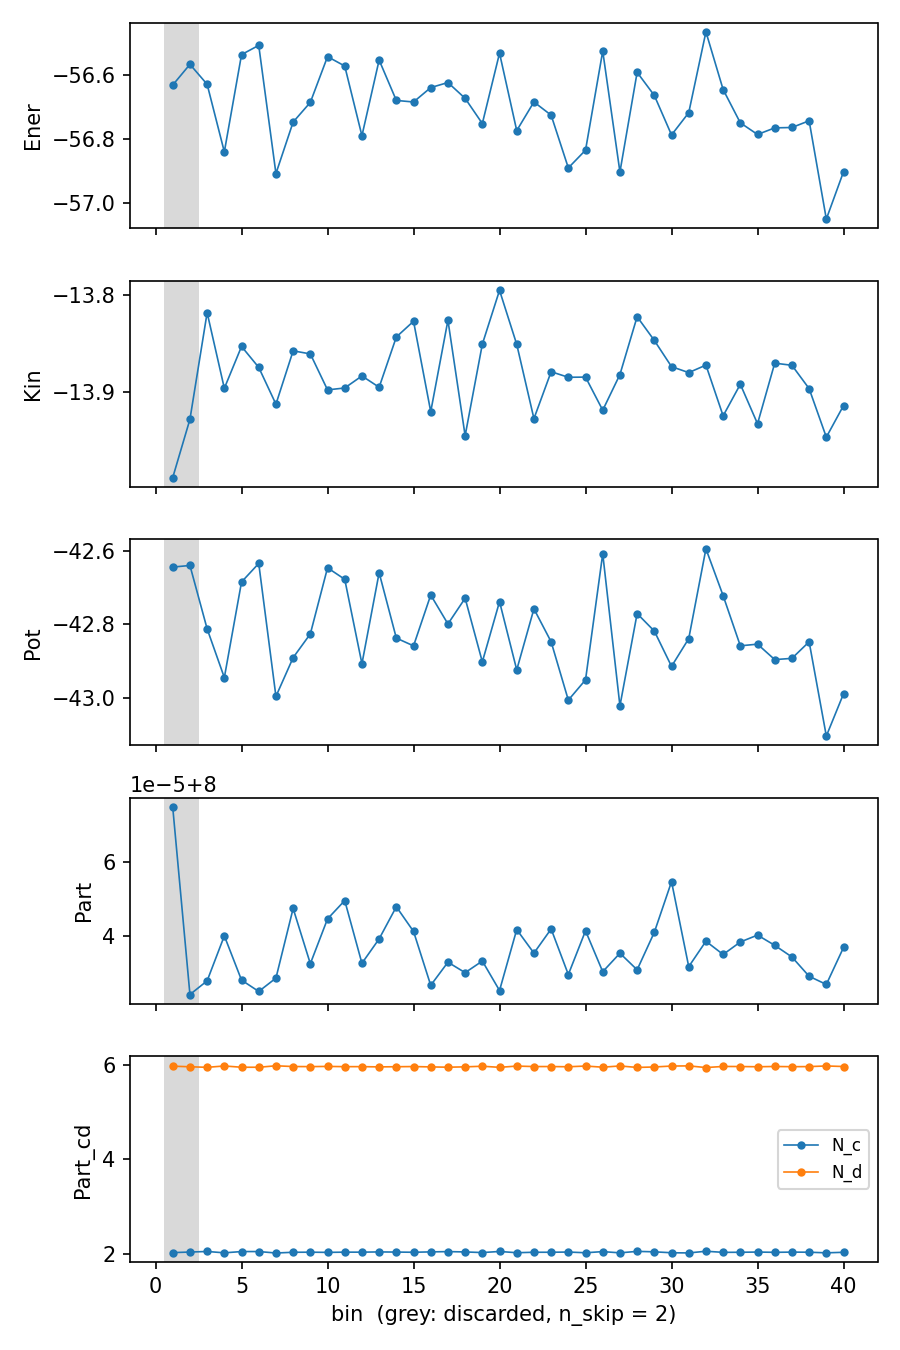
\includegraphics[width=0.45\textwidth]{figures/example_bins.png}
  \caption{\f{bins.png} for the Heisenberg $2\times2$ test: value of each bin. The grey area
  marks the \f{n\_skip} $=2$ discarded bins. Here the run is thermalised after one bin.}
  \label{fig:bins}
\end{figure}

\begin{figure}[t]
  \centering
  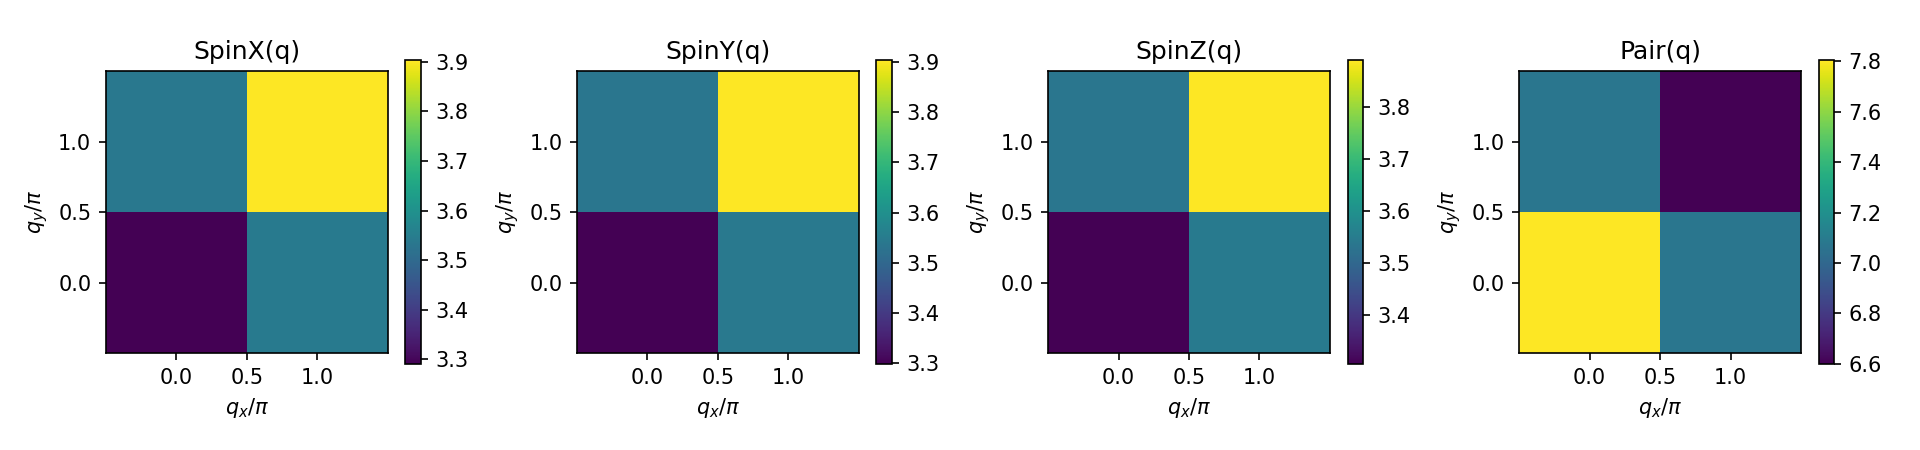
\includegraphics[width=\textwidth]{figures/example_Sq.png}
  \caption{\f{Sq.png} for the same run: structure factors on the $2\times2$ momentum grid. The
  spin structure factors peak at $(\pi,\pi)$ and are equal for $x,y,z$ (SU(2) symmetry); the
  pair structure factor peaks at $\mathbf q=0$.}
  \label{fig:sq}
\end{figure}

\subsection{\texorpdfstring{Extrapolation $\Delta\tau\to0$}{Extrapolation dtau -> 0}}
\label{sec:dtau}
Run the same parameters with several $\Delta\tau$, each in its own directory, e.g.\
$\Delta\tau=0.05, 0.025, 0.0125$. Then
\begin{lstlisting}
python3 $AN ~/QMC_runs/Heis_dt0.05 ~/QMC_runs/Heis_dt0.025 ~/QMC_runs/Heis_dt0.0125 --dtau
\end{lstlisting}
fits $O(\Delta\tau)=O_0+b\,\Delta\tau^2$ (weighted by the error bars) to every observable:
\begin{lstlisting}[basicstyle=\ttfamily\scriptsize]
  observable                 Dtau=0.05        Dtau=0.025       Dtau=0.0125               O_0 chi2/dof
  Ener                     -56.708(22)       -56.684(22)       -56.733(21)       -56.715(18)     2.42
  Kin                     -13.8793(60)      -13.6233(65)      -13.5628(75)      -13.5400(60)     0.10
  Pot                      -42.828(20)       -43.061(21)       -43.170(20)       -43.174(17)     2.28
  N_c                       2.0386(16)        2.0675(14)        2.0716(13)        2.0750(11)     2.02
  ...
\end{lstlisting}
The exact values are $\text{\f{Kin}}=-13.53681$, $\text{\f{Pot}}=-43.17951$, $N_c=2.07541$:
the $\Delta\tau=0.05$ values of \f{Kin} and $N_c$ are far off, while $O_0$ agrees within
$1\sigma$.

\subsection{Your own analysis in Python}
The functions in \f{analyze.py} can be imported:
\begin{lstlisting}[language=Python]
import sys; sys.path.insert(0, "/path/to/ALF_SZ/Scripts_and_Parameters_files/Hubbard_Sz")
import analyze as an

run = "/path/to/QMC_runs/Sz_L6_U1_b5"
E, dE, sign, _ = an.read_scalJ(run, "Ener")       # arrays of means and errors
qs, S, dS      = an.read_eqJK(run, "SpinZ")       # q points, S(q)[iq, o1, o2], errors
par            = an.read_parameters(run)          # dict of the namelist entries
bins, s        = an.read_scal_bins(run, "Ener")   # raw bins (Nbin, Nobs) and sign per bin
\end{lstlisting}
This is convenient for plotting observables against $U$, $\beta$ or $L$ over many run
directories. ALF also provides the more general Python package \emph{pyALF}
(\url{https://git.physik.uni-wuerzburg.de/ALF/pyALF}), which can read these directories as
well.

%=======================================================================================
\section{Validation: reference values}
\label{sec:validation}
%=======================================================================================

$2\times2$ lattice, $t=1$, $\delta=0.4$, $\mu=-2$, \f{Ham\_chem} $=0.3$, $U=1$, $\beta=2$,
$\Delta\tau=0.05$, $40$ bins of $200$ sweeps, \f{n\_skip} $=2$. These are the \f{parameters\_test\_2x2} files.
Details: \f{Infos/Test\_results\_Hubbard\_Sz.tex} and \f{Infos/Test\_results\_TwoBand\_Spin.tex}
in the project folder.

\begin{center}
\small
\begin{tabular}{lrrrr}
\toprule
 & \multicolumn{2}{c}{Ising (\f{Hubbard\_Sz})} & \multicolumn{2}{c}{Heisenberg (\f{TwoBand\_Spin})}\\
quantity & ED & QMC & ED & QMC \\
\midrule
\f{Ener}            & $-31.80783$ & $-31.8098(72)$ & $-56.71632$ & $-56.708(22)$ \\
\f{Part}            & $8.27457$   & $8.2675(27)$   & $8.00004$   & $8.0000359(12)$ \\
$N_c$               & $2.38350$   & $2.3771(26)$   & $2.07541$   & $2.0386(16)^{*}$ \\
$S^{zz}(\pi,\pi)$   & $3.74246$   & $3.744(27)$    & $3.91851$   & $3.8907(88)^{*}$ \\
average sign        & 1 & 1 & 1 & 1 \\
\bottomrule
\end{tabular}
\end{center}
$^{*}$Trotter error at $\Delta\tau=0.05$; agrees with ED after extrapolation
(Sec.~\ref{sec:dtau}).

%=======================================================================================
\section{Troubleshooting}
%=======================================================================================

\begin{description}
\item[\f{Environment variable ALF\_FC not set}] \f{make} was called without
  \f{source configure.sh ...} in the same terminal.
\item[\f{Not found: .../Prog/ALF.out}] ALF is not compiled; see Sec.~2.
\item[Model not recognised / namelist error] \f{ham\_name} and the name of the model namelist
  must match (\f{\&VAR\_Hubbard\_Sz} or \f{\&VAR\_TwoBand\_Spin}), and the model must be listed
  in \f{Prog/Hamiltonians.list}. A parameter that does not exist in the namelist stops the
  program; e.g.\ \f{Ham\_Int} in \f{\&VAR\_Hubbard\_Sz} gives
  \f{Fortran runtime error: Cannot match namelist object name ham\_int}. \f{run.sh} prints this
  line from \f{run.log}.
\item[Wrong model runs] Check which \f{ALF.out} you call. Only this ALF folder contains the
  new models.
\item[\f{Both plain text and HDF5 configuration present}] The run directory contains output
  of an HDF5 and a non-HDF5 build. Use a fresh directory.
\item[Results change when the run is continued] The parameter file was changed in between.
  Every run directory must correspond to one parameter set.
\item[\f{ana.out failed ... too few bins}] \f{ana.out} needs at least two bins after the
  \f{n\_skip} discarded ones. Continue the run (call \f{run.sh} again) to add bins.
\end{description}

\end{document}
